\documentclass[11pt,a4paper]{article}
\usepackage{termpaper}
\usepackage[utf8]{inputenc}
\usepackage{graphicx}
\usepackage{listings}
\usepackage{xcolor}
\usepackage{cleveref}
\usepackage{filecontents}
\usepackage{minted}
\usepackage{url}
\usepackage[labelfont=bf,textfont=it]{caption}

\definecolor{lstcolor}{rgb}{0.95,0.95,0.95}

\lstdefinestyle{customc}{
  belowcaptionskip=1\baselineskip,
  breaklines=true,
  frame=L,
  xleftmargin=\parindent,
  language=C,
  showstringspaces=false,
  basicstyle=\ttfamily\scriptsize,
  keywordstyle=\bfseries\color{green!40!black},
  commentstyle=\itshape\color{purple!40!black},
  identifierstyle=\color{blue},
  stringstyle=\color{orange},
  tabsize=2
}
\lstset{escapechar=@,style=customc}

\newminted{c}{tabsize=2,fontsize=\footnotesize,bgcolor=lstcolor,linenos,breaklines}
\newmintinline{c}{bgcolor=lstcolor, fontsize=\footnotesize}
\newmintedfile{c}{tabsize=2,fontsize=\footnotesize,bgcolor=lstcolor,linenos,breaklines}

%opening
\title{Parallel breadth-first search}
\author{
 \authorname{Alexander Gallauner} \\
 \studentnumber{1026090} \\
 \curriculum{534} \\
 \email{alexander.gallauner@gmail.com}
}

\begin{document}
\maketitle
\begin{abstract}
To have a continuous progress of the performance of processors, it was necessary to concentrate on the development of multicore processors. That development offered another problem. The programs or rather the algorithmic way of thinking have to be changed to get runtime enhancements with multicore processors. It is the job of the developers to split up the work from one core to many cores and to coordinate the communication between these cores. In this Bachelor thesis the focus is on algorithms for searching in graph data structures and how to parallelize these algorithms. To make it specific, we concentrate on the breadth-first search, because it is easier to parallelize than the depth-first search. First there is a presentation of a sequential algorithm to solve that problem. After that a parallel realization in pseudo code follows. We show the differences between the sequential and parallel solution and how the processors have to communicate in the parallel algorithm. After that we give an overview of different realizations and we show a low level implementation of our last version with some implementation details in the programming language C and the library OpenMPI. Additionally, we present the performance of the parallel solutions and how changes influence the runtime of them.
To get a feeling how good the solution is, we use our parallel algorithm in a benchmark for supercomputers called graph500. Graph500 establishes a large-scale benchmark for data-intensive supercomputer applications. With observing the rules of the graph500 project it is possible to compare the results of Jupiter with results of some other supercomputers, listed in the graph500 ranking.
\end{abstract}

\clearpage

\section{The breadth-first search - BFS}
\label{sec:breadth-first search}

The main application of the breadth-first search, illustrated by Cormen, Leiserson, Rivest and Stein \cite{cormen_introduction_2009}, is to find the shortest path between two nodes, in our case the root node and a successor node, measured by the number of edges between these two nodes. In comparison to that the path that is found by a depth-first search can be any path. It is not guaranteed that it is the shortest one.

\subsection{Sequential BFS}
\label{sec:sequential-bfs}

\begin{listing}[h]
\begin{ccode}
/*
input: adjacency buffer, root node
output: parent array
*/
BFS(adj_buffer, root){
	set_level(level, root);
	while level has nodes {
		for each Node n in level {
			neighbours = get_neighbours(adj_buffer, n);
			for each Node m in neighbours{
				set_level(next_level, m);
				set_parent(parents, n, m);
			}
		}
		level = next_level;
		clear(next_level);
	}
	return parents;
}
\end{ccode}
\caption{Sequential algorithm of the BFS.}
\label{lst:seq}
\end{listing}

The sequential BFS (breadth-first search) algorithm in Listing~\ref{lst:seq} is not difficult to understand. Input is an adjacency buffer, which stores the neighbors of each vertex in the graph, and the vertex identifier of the root node. Additionally there is an array necessary, which stores the index referred to the adjacency buffer for each node. But that is not important for understanding the algorithm, it will be explained in Section~\ref{sec:impl_details}. So there is no extra field given in the input parameters. \\
We can split the graph into levels, each level is handled in one single iteration of the BFS. In other words the level is the length of the path from the root node to all nodes of a specific level.
Then there starts the first round of the BFS. We take all nodes (root node for the first level) of the current level (that is level 0) and visit all neighbors of the nodes of the current level. All neighbors that have been visited are now the nodes of the next level (in this case that is level 1). The next step is to take all nodes of level 1 and visit all neighbors of these nodes. The BFS algorithm ends if the current level has no neighbors anymore. Output of the algorithm is a parent array, which saves the vertex identifier of the parent node for each vertex of the graph. For that reason it is called parent array.

\subsection{Parallel BFS}
\label{sec:parallel-bfs}

\begin{listing}[h]
\begin{ccode}
/*
input: for each processor - adjacency buffer of assigned nodes, level information
output: parent array
*/
BFS_PAR(adj_buffer, level){
	while level has nodes {
		for each Node n in level {
			neighbours = get_neighbours(adj_buffer, n);
			for each Node m in neighbours{
				set_level(next_level, m);
				set_parent(parents, n, m); 
			}
		}
		level = synchronize(next_level);
		clear(next_level);
	}
	return parents;
}
\end{ccode}
\caption{Parallel algorithm of the BFS.}
\label{lst:parallel}
\end{listing}

To run an implementation of an algorithm on a distributed memory system, the main problem is to split the work of the sequential algorithm into smaller pieces and assign that pieces of work to the existing processors of the system which are in use. The first approach of splitting the BFS is to split the nodes of each level to the processors. Every processor of the system just visits the neighbors of the nodes which were distributed before to that processor. The problem with this approach is that the communication costs are pretty high, because it is necessary to distribute the nodes and edges every round (level) of the BFS algorithm.\\
So the second and also chosen approach, illustrated in Listing~\ref{lst:parallel}, is to distribute all the existing nodes and corresponding edges of the graph to the processors. With that approach the highest amount of communication is before the algorithm starts. After that the processors have to communicate in such a way, that they know which nodes are in the next level. But that is less information to distribute than to distribute plenty of nodes and edges in every iteration of the algorithm.\\
So the function \cinline/BFS_PAR/ of Listing~\ref{lst:parallel} is called from every involved processor of the system with the adjacency buffer of the assigned nodes and a level information as input. The structure of the level information can be neglected at this point, but the structure will be handled in the different implementations/versions in Section~\ref{sec:implementations} and Appendix~\ref{sec:versions}, but it is important that this data structure saves the information which nodes are in the current level. The structure of the level information and the relating synchronization of the level information, symbolized with \cinline/level = synchronize(next_level)/ in Listing~\ref{lst:parallel}, influences the runtime of the implementation extremely. The neighbors of the actual nodes are marked for the next round in another data structure, the next level data structure, which can be the same as the level structure. With the synchronization of the next level information the processors know which nodes they have to handle in the next round. For that reason the synchronized next level data structure is saved in the level data structure which is the input for the next round.\\
Output of this algorithm is a parent array again. What is not evident, but can be necessary, is the synchronization of the parent array. 

\section{Implementations of the parallel breadth-first search}
\label{sec:implementations}

In this section there is a presentation of different realizations of the algorithm of Section~\ref{sec:parallel-bfs}. We show three different versions how this parallel concept can be implemented. The third and last version is the version that fits the requirements best, so it is explained in a more detailed way and is also used in the implementation of the graph500 project. We always assume that the number of nodes and the number of processors are a power of two. With that assumption we can ensure that all processors have the same number of nodes and it is easier to work with bitmaps. Also the synchronization between the processors is quite easier.\\
The source code of any version can be found in Appendix~\ref{sec:versions}.

\subsection{First version - level bitmap}
\label{sec:firstversion}

At the beginning the first idea was to solve the breadth-first search problem with matrices where each element represents an edge between two nodes, like Buluç and Madduri did in a specific way in their research paper \cite{matrices}. The problem with that approach is that if there is a sparse matrix there is a high waste of memory, so we developed a solution which better fits our requirements.\\
It was our next idea to save only the edges that are existing and to leave out the rest. We decided to store all existing edges in a buffer and to work with an index array to find the edges of each node. So the next important question was if every processor has his own part of the buffer how should each processor share the information which nodes are in the current or next level of the BFS. So we came to the first version of the BFS implementation.\\
The first version of the algorithm is very similar to the algorithm in Listing~\ref{lst:parallel} and is characterized by a level and next level bitmap. Every node that is assigned to the processor has a bit in this level bitmap. If the bit is set it signalizes that the node belongs to the actual level. So the level bitmap has the information which nodes are active.\\
At every round of the algorithm, where all nodes of the actual level should be handled, each processor has to iterate over the level bitmap and checks if a bit is set or clear. If the bit is set, the processor iterates over the neighbours of this active node. That can be achieved with an array like \cinline/adj_buffer/ from Listing~\ref{lst:parallel}, where all neighbours of the to the processor assigned nodes are saved. Now we make use of the next level bitmap, where all bits are clear at the beginning of each round. If a node is active and we iterate over the neighbours, each neighbour is set in the next level bitmap. The next level bitmap has a size of \(n\) bits where \(n\) is the count of nodes of the whole graph. That is necessary because we also have to set bits of nodes that are not assigned to the specific processor. The nodes that are set in the next level bitmap will be the active nodes in the next round of the algorithm.\\
The following step is to synchronize the next level bitmaps of every processor. If there are \(m\) processors the \(m\) bitmaps are taken, a bitwise OR operation is executed on them and then dependent on the assigned nodes of each processor the right part of the synchronized next level bitmap is returned to the processors and is used as the level bitmap for the next round. In short the used synchronization operation can also be called reduce scatter operation, because there are many buffer or arrays gathered and then reduced to one with a reduction operation like the bitwise OR. After that reduction the information is scattered again.\\
That solution of the parallel breadth-first search has very good results as we can see in Section~\ref{sec:testingall}. The only problem with that approach is that it is difficult to add the functionality that it is possible to create an parent array and return it as a result of the implementation. Every try to add this functionality would make this approach inefficient.

\subsection{Second version - \cinline/uint64_t/ level array}
\label{sec:secondversion}

In the second version of the algorithm we used arrays instead of bitmaps. Every to the processor assigned node has a \cinline/uint64_t/ field in the level array, which has the same functionality as in Listing~\ref{lst:parallel}. In addition to that the next level bitmap is also replaced with a next level array of type \cinline/uint64_t/. The type \cinline/uint64_t/ is used because we set the rule that we want to save nodes with a vertex identifier up to \(2^{64}-1\). That is not necessary if we have a graph with a number of nodes under \(2^{32}\), but this requirement should be accomplished because it is later a requirment for the graph500 project where at least 6 bytes (48 bits) have to be allocated for identifying a node.\\
The important difference is that when we iterate over the neighbours through the array \cinline/adj_buffer/ we do not just flip a bit, we save the vertex identifier of the actual node, which is assigned to the current processor, as the parent of the neighbour in the next level array. After all processors iterate over their nodes and set all neighbours of the active nodes in the next level array, the next level array must be synchronized. That is done like in the first version in Section~\ref{sec:firstversion}, but another reduction operation is used. Instead of \cinline/MPI_BOR/ the reduction operation \cinline/MPI_MAX/ is used. The reason for that is that we now have multiple arrays that have to be reduced to one and these arrays have the vertex identifier of the parent for each node in their fields. \cinline/MPI_MAX/ takes for instance the field on position 0 of every input array and chooses the field with the highest number, the maximum, as result. This procedure is continued till the field with the last position is reached. With that strategy the race condition can be solved that one node is visited in the same level from two different nodes. Then \cinline/MPI_MAX/ chooses the node with the higher vertex identifier and set this node as parent.\\
After reducing the arrays to one array the right part of this synchronized array is scattered to the processors and assigned to the local level array. In the next round of the algorithm the processor iterates over the level array. If a field of the level array is unequal to zero and there is not a parent saved before for this node, the vertex identifier of the parent is adopted and saved in a local parent array.\\
With this approach of solving the parallel breadth-first search we meet all requirements, but like it is shown in Section~\ref{sec:testingall} it is very inefficient because reducing the next level arrays of type \cinline/uint64_t/ in each round is really time-consuming and becomes more sophisticated with the increasing number of processors.

\subsection{Third and current version - visited bitmap}
\label{sec:thirdversion}

The basic idea of this approach is that we do not have a next level bitmap or array, we always keep a bitmap of all visited nodes in all levels synchronized. All processors know which node is already visited and which not and the parent of each node can be correctly stored at each processor. Before the algorithm ends the parent arrays of each processor are reduced to one parent array. Section \ref{sec:core} gives a good overview for this approach. Low-level implementation details can be found in Section~\ref{sec:impl_details}.

\subsubsection{Overview of the third version}
\label{sec:core}
\begin{listing}[h]
\begin{ccode}
/*
input: every proc has adjacency buffer of owned nodes, visited_bitmap where root is set to one
output: parent array
*/
void* BFS(adj_buffer, visited_bitmap){
	char oneChildisVisited = 1;
	while (oneChildisVisited){
	oneChildisVisited = 0;
	for (i = 0; i < size(nodes_owned); i++){
		if (nodes_owned[i] is visited for the first time) {
			neighbours = get_neighbours(adj_buffer, nodes_owned[i]);
			for (j = 0; j < size(neighbours); j++){
				if (neighbours[j] is not visited) {
					oneChildisVisited = 1;
					set_visited_bitmap(visited_bitmap, neighbours[j]); // sets the visited bitmap on position of neighbour[j] to 1
					save_parent(parent_array, nodes_owned[i]+1,neighbours[j]); // saves that nodes_owned[i]+1 is parent of neighbours[j] in parent array
				}
			}
		}	
	}
	synchronize(oneChildisVisited);
	if (oneChildisVisited){
		sychronize(visited_bitmap);
	}
	return parent_array;
}
\end{ccode}
\caption{Parallel BFS in more detail.}
\label{lst:detailedparallel}
\end{listing}
As Listing~\ref{lst:detailedparallel} shows, there are two input parameters. The first one is the adjacency buffer, like mentioned in Section~\ref{sec:sequential-bfs}. The second parameter, called \cinline/visited_bitmap/, is a bitmap with a size of the involved nodes in the breadth-first search. If a bit on position \(n\) in the bitmap is set (1) it means that the node with the identifier \(n\) is visited, otherwise a bit that is clear (0) stands for unvisited. So this bitmap gives the information which nodes are visited already and which nodes not. Additionally to that \cinline/nodes_owned/ represents an array of nodes, which are assigned to the specific processor.\\
Important is the flag \cinline/oneChildisVisited/. This flag keeps the information, if there is any new node visited at any processor and is synchronized at line 21. The \cinline/synchonize(oneChildisVisited)/ operation means that there are all \cinline/oneChildisVisited/ chars taken and then a bitwise OR is performed on these chars. If the reduced char variable is set (1), the \cinline/visited_bitmap/ will be synchronized with \cinline/synchronize(visited_bitmap);/.\\
So if the processors communicate through \cinline/oneChildisVisited/ that there is at least one new visited node for the next round, the processors have to iterate over the assigned nodes and check if there is one of them set in the \cinline/visited_bitmap/ and not visited in a iteration before. The checking if a node or vertex is visited already is not handled in this Section and can be implemented in multiple ways. If there is a node which is not visited before and the bit in the \cinline/visited_bitmap/ related to that node is set, then the algorithm iterates over the neighbours of that node, where the obtaining of the neighbours of a node is simplified with \cinline/get_neighbours(adj_buffer, nodes_owned[i])/. If the neighbour is visited for the first time, the bit of that node is set in the \cinline/visited_bitmap/ and the processor saves the parent of that neighbour in the \cinline/parent_array/. If the node with the vertex identifier \(n\) is parent of the node with vertex identifier \(m\), then the number \(n\) is stored on position \(m\) in the \cinline/parent_array/. After checking all nodes, there have to be a synchronization like mentioned before in this section. First the \cinline/oneChildisVisited/ is synchronized and dependent on that there is a synchronization of the \cinline/visited_bitmap/. After the synchronization of the \cinline/visited_bitmap/ it is important that all processors have the same bitmap, where all bits of nodes that are visited in the iterations before from any processor are set. 

\subsubsection{Implementation details}
\label{sec:impl_details}

In this section there is an explantion of the algorithm in Section~\ref{sec:core} with low level implementation details. The programming language is C and we make use of the OpenMPI library. A good basic description of MPI is given by Rauber and R{\"u}nger \cite{rauber}. \\
Let us start with the function declaration of the BFS function. There are more parameters necessary than in Listing~\ref{lst:detailedparallel}.
\begin{ccode}
void bfs(uint64_t *visited_bitmap, uint64_t *adj_buffer, uint64_t adj_buffer_size, uint64_t *index_of_node, int my_rank, int procs, int scale, uint64_t *parent_array);
\end{ccode}
\cinline/visited_bitmap/ is a bitmap of type \cinline/uint64_t/ and contains the information, which nodes of the entire graph are visited and which not. \cinline/uint64_t/ is an integer type and is equal respectively to unsigned long long. The important fact of this type is that we can set 64 bits in one value. \\ 
\cinline/adj_buffer/ is an array and saves the neighbours of the nodes, which are assigned to the processor that is calling the function. For \cinline/adj_buffer/ we also use the data type \cinline/uint64_t/ to address vertex identifiers up to a number of \(2^{64}-1\). The parameter \cinline/index_of_node/ is a helper array with a size of the to the processor assigned nodes. Each entry of \cinline/index_of_node/ stores an index of the array \cinline/adj_buffer/ and therefore the indices, where the neighbours of the nodes are located in the \cinline/adj_buffer/. \\
The parameters \cinline/my_rank/ and \cinline/procs/ contain the processor identifier and the number of working processors. Dependent on the processor identifier \cinline/my_rank/ the graph, in particular the nodes and edges, is scattered to the processors.\\
With the parameter \cinline/scale/ the number of nodes can be calculated that are assigned to the processor. The result of \(2^{scale}\) is the number of nodes of the entire graph. If it is divided by the number of working processors, the result is the number of nodes that are assigned to one processor. To ensure that all processors have the same number of nodes we always use a power of two for the number of vertices of the graph and the number of working processors. \\
The last parameter \cinline/parent_array/ is the result of this algorithm. \\
After checking if there is at least one new visited node in the actual level, every processor iterates over the bitmap \cinline/visited_bitmap/ which is synchronized over all processors. The processors iterate over different parts of the \cinline/visited_bitmap/ dependent on the processor identifier \cinline/my_rank/. For each node that is assigned to the processor there must be a check if it is visited for the first time.\\
So the pseudo code line
\begin{ccode}
if (nodes_owned[i] is visited for the first time){
\end{ccode}
can be written in C in that way
\begin{ccode}
position = (uint64_t) pow(2, (i % 64));
if (position & visited_bitmap[((nodes_owned_count*my_rank+i) / 64)] & ~visited_local[(i / 64)]) {
\end{ccode}
We need \cinline/position/ to target a specific bit in a value of type \cinline/uint64_t/. As mentioned before we can set 64 bits in one variable or field. To get the position of a node in a bitmap, we have to calculate two to the power of \(i\) where \(i\) is the vertex number of the specific node modulo the count of possible bits, which is 64 in our case. Keep in mind that the vertex number is not the unique vertex identifier. The vertex number is on every processor between zero and the number of assigned nodes. It is possible to calculate the unique vertex identifier with the local vertex number and the processor identifier \cinline/my_rank/. The unique vertex identifier is calculated with \cinline/nodes_owned_count*my_rank+i/. This calculation is necessary to get the absolute position of the node in the bitmap \cinline/visited_bitmap/. So if the unique vertex identifier is divided by the count of bits of one value, we get the correct field of the bitmap \cinline/visited_bitmap/. Let us show that with the example of node number 90 and with two processors where each processor has 256 nodes. There must be a bitmap \cinline/visited_bitmap/ with \(512/64 = 8\) fields and our node with vertex number 90 at the processor with the processor identifier 0 must be at field number \((256*0+90) / 64 = 1\).\\
Additionally we have a local bitmap \cinline/visited_local/, which only needs the local vertex number to calculate the correct field. The bitmap \cinline/visited_local/ is individual for every processor and saves the information which nodes are already visited in the levels or iterations before. That is similar to the bitmap \cinline/visited_bitmap/, but in comparison to \cinline/visited_bitmap/ the new nodes of the actual level are not set in \cinline/visited_local/. So it is possible to get the new nodes of the actual level with a bitwise AND operation \cinline/&/ between the position of the specific node, the global \cinline/visited_bitmap/ and the inversion of the local bitmap \cinline/visited_local/.\\
Assuming that the node was not visited before and the condition is true, we iterate over all neighbours of that node. We get the neighbours of a node through the array \cinline/adj_buffer/ and the helper array \cinline/index_of_node/. If we have a node with the vertex number \(i\) we get the index for the \cinline/adj_buffer/ with \cinline/index_of_node[i]/. Beginning there we iterate over the \cinline/adj_buffer/ until we reach the index \cinline/index_of_node[i+1]/. 
For every neighbour there must be a check that the neighbour was not visited before. That was handled in Listing~\ref{lst:detailedparallel} with \cinline/neighbours[j] is not visited/. With bitmaps it looks like this:
\begin{ccode}
position = (uint64_t) pow(2, (adj_buffer[j] % 64));
if (position & ~visited_bitmap[(adj_buffer[j] / 64)]){
\end{ccode}
Firstly we need the position of the neighbour with the vertex identifier \cinline/adj_buffer[j]/. Secondly there is a check if the neighbour is already visited through a bitwise AND between the position and the inversion of the \cinline/visited_bitmap/.
If the condition evaluates to true the following code is executed
\begin{ccode}
parent_array[adj_buffer[j]] = (uint64_t) nodes_owned_count*my_rank+i+1;
visted_bitmap[(adj_buffer[j] / 64)] = visited_bitmap[(adj_buffer[j] / 64)] | position;
oneChildisVisited = 1;
\end{ccode}
which replaces the pseudo functions \cinline/set_visited_bitmap/ and \cinline/save_parent/ from Listing~\ref{lst:detailedparallel}. At first we save the parent of the neighbour \cinline/adj_buffer[j]/ in the array \cinline/parent_array/. For the identification of a parent the vertex identifier of the vertex number \cinline/i/ is saved and is calculated like before with \cinline/nodes_owned_count*my_rank+i+1/, but we add \(+1\) to the vertex identifier. That is because we want the number \(0\) for nodes in the \cinline/parent_array/ which do not have a parent. So if the node with the vertex identifier \(0\) is the parent of another node, we save \(1\) instead of \(0\) in the \cinline/parent_array/.\\
The next step is to set the bit in the bitmap \cinline/visited_bitmap/ on the position of the neighbour \cinline/adj_buffer[j]/. In addition to that the flag \cinline/oneChildIsVisited/ is set. With these steps we lay the foundation for the next round of the algorithm where the nodes of the next level are handled.\\
To share the information which nodes should be handled in the next round we have to synchronize the flag \cinline/oneChildisVisited/ and the bitmap \cinline/visited_bitmap/. That is done with
\begin{ccode}
MPI_Allreduce(MPI_IN_PLACE, (void *) &oneChildisVisited, 1, MPI_CHAR, MPI_BOR, MPI_COMM_WORLD);        
if (oneChildisVisited){
        MPI_Allreduce(MPI_IN_PLACE, (void *) visited_bitmap, (pow(2,scale) / BITS), MPI_UINT64_T, MPI_BOR, MPI_COMM_WORLD);
}
\end{ccode}
Here we make use of the operation \cinline/MPI_Allreduce/ of MPI. In MPI we just work with processes, it is not necessary to have specific information about the underlying system which can be a distributed-memory or shared-memory system. The distribution of processes to the processors is not done by the programmer, it is done by the operating system and MPI implementation. It is also possible to use a resource manager like SLURM (REF!!!). With MPI a specific number of processes is executed, which have to share a communicator to have the possibility to communicate with each other.\\
If a MPI operation is used, it is necessary to specify a communicator which is \cinline/MPI_COMM_WORLD/ in our case. This communicator is a predefined one and contains all executed processes. So if this communicator is used, we communicate with all other processes.\\
In short the \cinline/MPI_Allreduce/ operation takes data of all processes, applies a specific reduction operation on that data and returns the result to every process. That MPI operation is blocking. That means that it waits for all processes, which share this communicator, till the processes reach this line of code. The first parameter requires a pointer to a buffer that should be part of the operation. This is \cinline/MPI_IN_PLACE/ in our case, what means that we use the same buffer for input and output of the operation. So with \cinline/MPI_IN_PLACE/ we refer to the buffer of the second parameter. The second parameter specifies the location where the result should be stored. In our implementation \cinline/&oneChildisVisited/ and \cinline/visited_bitmap/ serve as input and output buffers. The third parameter gives the information how many elements should be taken from the buffer of the type that is specified in the fourth parameter. \cinline/MPI_BOR/ is our reduction operation in both cases and stands for the bitwise OR operation. A requirement for a reduction operation is that it takes any number of input values and returns one output value. We used the reduction operation \cinline/MPI_BOR/ in our implementation because we want a bitmap as result where every bit on a position is set which was also set in one of the input bitmaps on that position. That result bitmap is used in the next round of the algorithm where the nodes of the next level are handled.

\subsubsection{Algorithm analysis}
\label{sec:analysis}

While the sequential breadth-first search has a time complexity of \(\mathcal{O}(n + e)\), where \(n\) is the number of nodes and \(e\) is the number of edges, the time complexity of the third parallel implementation is different. In every round or level of the algorithm the processors have to iterate over all nodes that are assigned to them and check if they were visited in the last round. In the sequential solution it is sufficient to iterate over the nodes that are in the current level, but that is not possible in the parallel solution, because we work with other data structures. There results a time complexity of \(\mathcal{O}(dn + e)\) in the parallel solution. \(d\) defines the diameter of the graph and is the greatest distance between any pair of vertices.\\
Both the sequential and the parallel solution occupy \(\Theta(n + e)\) space in memory. If the sequential algorithm used an adjacency matrix instead of a list, the sequential algorithm would have a space complexity of \(\Theta(n^{2})\).

\section{Testing the implementations on Jupiter}
\label{sec:testingall}

For better understanding how manipulations in the algorithm influence the speed of the algorithm we compare the results of the different versions on Jupiter.
Jupiter is a distributed-memory system with the following description:
\begin{flushleft}
\begin{tabular}{| l |}
  \hline
  36 nodes x 2 x AMD "magny cours" 8-core Opteron 6134 processors \\
  32 GB main memory per node with 2.3 GHz\\
  \hline
\end{tabular}
\end{flushleft}
That means that there is a total number of 576 cores available and a total memory of 1152 GB. For testing we used OpenMPI version 1.10.3. Jupiter uses a workload manager, called SLURM. The version of SLURM that is used is 16.05.3.\\
The focus of this Section is testing and timing the parallel breadth-first search, not the things that have to be done to generate the graph and to get the adjacency buffer that is delivered to the BFS function. The graph generation can be done in multiple ways, but in our case it is generated by a Kronecker graph generator. Kronecker graphs were researched, among others, by Leskovec, Chakrabarti, Kleinberg, Faloutsos and Ghahramani~\cite{kronecker}.\\
In the following figure we work with a graph size of \(2^{25}\) nodes and \(2^{27}\) undirected edges. In short we just say that the graph has a scale of 25 and an edgefactor of 4. The number of processes is also a power a two, to ensure that all processes have the same number of nodes. For identifying a node there are 8 bytes (64 bits) allocated in all data structures. That means that the adjacency buffer \cinline/adj_buffer/, which is input of the BFS function and represents the graph, is of type \cinline/uint64_t/ in all versions of the algorithm. The bitmaps have also the type \cinline/uint64_t/, but that has the reason that we want to set 64 bits in one value.\\
After scattering the adjacency buffer to all processes the timer starts and ends when the processes do not have found any new nodes and have synchronized the parent array.\\
\begin{figure}[!ht]
   \centering
   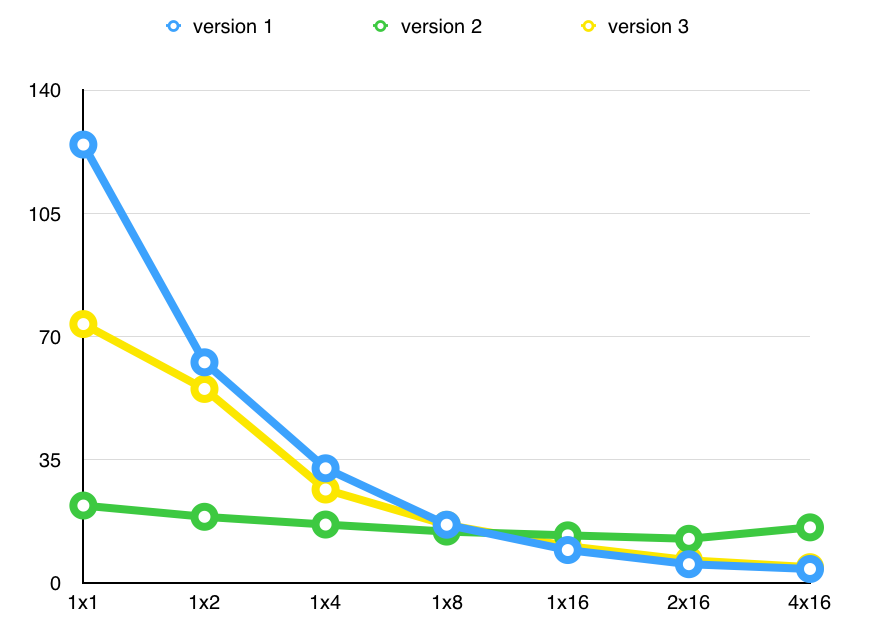
\includegraphics[width=1.00\textwidth]{allversions}
   \caption{Results of timing all versions of the breadth-first search. The x-axis defines the MPI processes in that way that we know how many cores of each node are used.Version 3 is not the fastest solution, but it is really close to version 1 and fits the requirements in a better way.}
   \label{fig:allversions}
\end{figure}
Figure~\ref{fig:allversions} shows the results of all three versions. We used different configurations of Jupiter to test the different versions. A configuration is characterized by the number of nodes and the number of cores that are used of each node. So if we write \(2x16\) it means that we use 2 nodes and 16 cores of each node. Altogether we have 32 processes in that example.\\
Version 1 has a quite good speedup with a higher number of cores, but the problem, like mentioned in Section~\ref{sec:firstversion}, is that we do not have a parent array at the end of this algorithm and it is hard to extend this approach to get one.\\
The implementation of Version 2 has a very bad speedup with the raising number of cores. Reason for that bad speedup is the synchronization of the next level array of type \cinline/uint64_t/. It takes too much time to reduce the entries of the next level array with the reduction operation \cinline/MPI_MAX/. In Table~\ref{tab:reducescatter} it is shown how much time the synchronization consumes for the different count of processes.\\
\begin{table}[!ht]
	\centering
	\begin{tabular}{ | l | l |}
  		\hline
  		Number of processes & Time for synchronization \\ \hline
  		1x1 & 3.41s \\ \hline
		1x2 & 9.61s \\ \hline
		1x4 & 10.76s \\ \hline
		1x8 & 11.1s \\ \hline
		1x16 & 12.0s \\ \hline
		2x16 & 13.5s \\ \hline
		4x16 & 14.2s \\ \hline
	\end{tabular}
	\caption{Total time for synchronizing the next level arrays.}
  	\label{tab:reducescatter}
\end{table}
The third version is a compromise between the first and the second version. On the one hand we want to synchronize as little as possible like in the first version. On the other hand, to get a parent array at the end of the algorithm, we have to synchronize more information than in the first version, but as we see in Table~\ref{tab:reducescatter} synchronizing the next level array of all nodes with the \cinline/MPI_MAX/ operation is too time-consuming. So we decide to reduce a bitmap of all nodes of the graph with the reduction operation \cinline/MPI_BOR/ and we get pretty good results with that decision.

\section{The graph500 project and my own realisation}
\label{sec:graph500}

The graph500 \cite{graph500} is a benchmark of supercomputer systems and concentrates on data intensive loads. Instead of counting double precision floating-point, the benchmark stresses more the communication between the nodes of the system. There are two kernels in this benchmark which are important for the computation and are timed. The first kernel has to generate a graph from a given edge list. In the second kernel there are 64 breadth-first searches from different start nodes. The start nodes are not choosed arbitrarily, they have to be randomly sampled. For each start node there have to be a computation of a parent array.\\
\\
\begin{listing}[H]
\begin{ccode}
/*
input: scale and edgefactor
output: performance information
*/
void graph500_benchmark(scale, edgefactor){
	edge_list = generate_edges(scale, edgefactor);
	buffer = kernel_1(edge_list, pow(2,scale)*edgefactor); // timed
	keys = generate_keys(scale, 64);
	performance_information = kernel_2(buffer); // timed
	print(performance_information);
}
\end{ccode}
\caption{Graph500 benchmark in pseudo code.}
\label{lst:graph500}
\end{listing}

Before the first kernel starts there is a generation of the edge list with a Kronecker generator, as illustrated in Listing~\ref{lst:graph500} through \cinline/edge_list = generate_edges(scale, edgefactor);/. The most important thing in this function is that there is a generation of undirected edge tuples which must not show any locality that can be exploited by the timed kernels. Our implementation of the Kronecker generator takes the two parameters \cinline/scale/ and \cinline/edgefactor/ and has the initiator parameters specified in Table~\ref{tab:kronecker}.\\
\begin{table}[h]
	\centering
	\begin{tabular}{ | l | r |}
  		\hline
  		0.57 & 0.19 \\ \hline
  		0.19 & 0.05 \\ \hline
	\end{tabular}
	\caption{Initiator parameters for the Kronecker generator}
  	\label{tab:kronecker}
\end{table}
That means that each edge has a specific probability to belong to the corresponding quarter of the adjacency matrix. This procedure needs some iterations, more precisely \cinline/scale/ iterations to generate one edge.
After that the computation of the graph, which is later used in kernel 2, follows.
\begin{ccode}
buffer = kernel_1(edge_list, pow(2,scale)*edgefactor);
\end{ccode}
This step is timed, so it is important that it is done as fast as possible. But the fastest solution is not always the best one, because the computed graph from kernel 1 must be also useable for kernel 2 in an appropriate way.\\
Our solution for kernel 1, shown in Listing~\ref{lst:kernel1}, is that we sort the edge list ascending by vertex identifier, first by the start vertex identifier second by the end vertex identifier.
\begin{listing}[H]
\begin{ccode}
/*
input: edge list and count of edges
output: adjacency buffer and scale
*/
int kernel_1(edge_list, edges, *buffer){
	scatter(edge_list); // before sorting the edge list is scattered
	sort(edge_list);
	tree_merge(edge_list); //the sorted edge list is merged in a tree based way
	if (rank == root){
		scale = calculate_scale(edge_list);
	}
	bcast(scale); // scale is broadcasted
	if (rank == root){
		bounds = calculate_bounds(edge_list);
	}
	scatter(bounds);
	scatter(edge_list); //now the sorted edge list is scattered
	adj_buffer = create_buffer(edge_list); //each proc creates the buffer from the received edge list
	return scale;
}
\end{ccode}
\caption{Kernel 1}
\label{lst:kernel1}
\end{listing}
The sorting of the edge list is done in parallel with a Quicksort-Merge implementation to get a good performance for the first kernel. We choose the sorting algorithm Quicksort (REF), because it is a efficient sorting algorithm, particularly and that is important, in average case. The procedure is to scatter the edge list to the processors and every processor does the Quicksort on the received edge list. The next step is to merge the different sorted edge lists in a way, that the processor with identifier 0 has the whole sorted edge list at the end. Instead of calling the merge operation \(p\) times in sequential order, where \(p\) is the number of processors, we decided to implement a tree based merging of the edge lists, like Puneet Kataria presented in his work \cite{quickmerge}.\\
With the sorted and merged edge list the \cinline/scale/ or rather the number of nodes is calculated at the processor with identifier 0. The \cinline/scale/ is not known from the beginning. The implementation of the graph500 has to calculate it from the given edge list. So the processor with identifier 0 calculates this information and communicates it with the other processors. After that the sorted edge list is scattered to the processors. Every processor gets the edges of the nodes he owns, what is guaranteed with \cinline/bounds = calculate_bounds(edge_list);/ . For instance if we have 64 nodes and four processors then the first processor gets the edges with the start vertex from 0 to 15. The second processor gets the edges from 16 to 31, the third from 32 to 47, the last from 48 to 63. The processors can get a different count of edges dependent on the start vertex of the edges. We first send the processors the count of the specific edges with \cinline/scatter(bounds);/. Then the processor allocates memory for that edges and receives them. \\
With the splitted edge list the adjacency buffer, which will be used in kernel 2, is created in such a way that the buffer contains the end vertex entries of the received edges. Duplicate edges are eliminated. To know at which entry the edges of each node start, we need an additional array of the size of owned nodes. With that the first kernel is completed.\\
\begin{listing}[H]
\begin{ccode}
/*
input: buffer 
output: performance information
*/
char *kernel_2(buffer){
	keys = generate_keys(scale, 64);
	for each(Key k : keys){
		parent_array = BFS(buffer, k); // timed
		validate(parent_array);
	}
}
\end{ccode}
\caption{Kernel 2}
\label{lst:kernel2}
\end{listing}
For the second kernel, as illustrated in Listing~\ref{lst:kernel2}, there have to be a BFS search of 64 keys, which are randomly sampled. Firstly we generate the search keys with 
\begin{ccode}
keys = generate_keys(scale, 64);
\end{ccode}
One key stands for the vertex identifier of a node and the degree of that node must be at least one, not counting self-loops. That is a bit tricky in our solution because we do not save the degree of each node. So instead of iterating over the edge list for each randomly sampled key and checking the degree of that node we broadcast a message to all processors after generating a key. The processor that is responsible for that key counts the edges and gives an answer to the processor with the identifier zero, which is responsible for generating the keys. If the key is acceptable, the key will be one of the search keys. If not, the procedure will be repeated.\\
Secondly we iterate over them and compute a parent array for each search key \cinline/k/ with
\begin{ccode}
parent_array = BFS(buffer, k);
\end{ccode}
For the BFS search we use our solution from Section~\ref{sec:thirdversion}. To know if the computed parent array is correct, there is a validation after each BFS search. This validation is not timed and does not influences the performance output, so it is sequential in our solution.\\
Further informations and code details of our solution of the graph500 benchmark can be found in Appendix~\ref{sec:sourcecode}.

\section{Graph500 performance of Jupiter}
\label{sec:performance}

The performance of Jupiter is measured by Kernel 1, where the graph is generated from the input edge list, and Kernel 2, where 64 parent arrays are computed within a BFS search. Figure~\ref{fig:kernel1} shows the execution times in seconds of the first kernel. There are different graph sizes defined on the x-axis. The edgefactor is always 16. That means that we have 16 times more edges than nodes. Jupiter is configured in a way that we use 32 nodes and in the one case 8 cores and in the other case 16 cores of each node. The y-axis defines the seconds for kernel 1.

In contrast Kernel 2 is measured by the performance metric TEPS (traversed edges per second).  Let \(m\) be the number of input edge tuples within the component traversed by the search and \(t(n)\) be the execution time for Kernel 2. Then the normalized performance rate is: \(TEPS(n) = m / t(n)\)\\
Figure~\ref{fig:kernel2} shows the TEPS on the y-axis and the graph sizes on the x-axis. The scale of the graph goes from 12 to 22 and the edgefactor is 16, like in kernel 1. The configuration of Jupiter is equal to kernel 1.\\
\\
FIGURES FOLLOW:\\
Example of performance using 8 nodes and 8 cores each:\\
Time for reading the graph: 73.006943\\
Time for generating edge buffer, sorting and scattering: 17.026062\\
Time for bfs searching: 679.820026\\
GTEPS: 0.006318\\

\section{Summary}
\label{sec:summary}



\clearpage

\nocite{*}
\bibliographystyle{abbrv}
\bibliography{bachelor}
\clearpage
\appendix
\section{BFS versions}
\label{sec:versions}
\lstinputlisting[firstline=138,lastline=196,caption={Version 1 - level bitmap},label=version1]{../Source/bfs_par.c}
\lstinputlisting[firstline=135,lastline=183,caption={Version 2 - level array},label=version2]{../Source/bfs_par_parentarray.c}
\lstinputlisting[firstline=153,lastline=205,caption={Version 3 - visited bitmap},label=version3]{../Source/bfs_par_allvisited_parallelsort.c}
\section{Source Code - graph500}
\label{sec:sourcecode}
\lstinputlisting[caption={BFS solution},label=bfs]{../Source/bfs_par_allvisited_parallelsort.c}
\clearpage
\lstinputlisting[caption={Kronecker Generator},label=kronecker_generator]{../Source/kronecker_generator.c}
\clearpage
\lstinputlisting[caption={project.h},label=project]{../Source/project.h}

\clearpage


\end{document}